\documentclass[12pt, a4paper, onecolumn, oneside, toc=bibliographynumbered, liststotoc]{scrartcl} %Schriftgröße 12pt, DIN A4, 1 Spalte, einseitig bedruckt, Literaturverzeichnis in Inhaltsverzeichnis eintragen mit Nummerierung als Anhang

\usepackage[T1]{fontenc} %Codierung für deutsche Schriftzeichen
\usepackage[utf8]{inputenc} % UTF-8 Encoding
\usepackage[ngerman]{babel} % Neue Deutsche Rechtschreibung
\usepackage[onehalfspacing]{setspace} %1,5 Zeilen Zeilenabstand
\usepackage{scrlayer-scrpage} %Kontrolle von Fuß- und Kopfzeile
\usepackage{graphicx} %Einfügen von Bildern
\usepackage{pdfpages}
\usepackage{float}
\usepackage[printonlyused, nohyperlinks, smaller]{acronym} %Unterstützung für Abkürzungen und Abkürzungsverzeichnis - es werden nur verwendete Abk. gedruckt
\pagestyle{scrheadings} %Seitenstil
\chead*{\pagemark} %Kopfzeile Mitte - Seitenzahl
\cfoot*{} %Fußzeile Mitte - leer
\usepackage[german=quotes]{csquotes}
\usepackage[backend=bibtex, citestyle=authoryear, bibstyle=authoryear, sorting=nty]{biblatex} %Angaben für Zitate - Nutzt Bibtex, Markierung auf Seite als alphanumerische Abkürzung, Sortierung nach Auftreten
\addbibresource{Aufgabe_1.bib} %Bibliotheksdatei
% !!! Um Bibtex richtig zu verwenden, nach jeder Änderung in der .bib-Datei Bibtex laufen lassen !!!

%\setcounter{tocdepth} {4} % Inhaltsverzeichnis bis subsubsection
%\setcounter{secnumdepth}{4} % Nummerierung des Inhaltsverzeichnis bis subsubsection

\begin{document}
%Titelblatt und Inhaltsverzeichnis
\pagenumbering{roman} %Seitennummerierung i, ii, iii etc. 
	%Angaben für Maketitle
	\titlehead{Hochschule Rhein-Waal \\ %Hochschulinformationen
	Fakultät: Kommunikation und Umwelt\\
	Studiengang: Verwaltungsinformatik\\
	Modul: Workshop 2: Wissenschaftliches Schreiben\\}
%	\subject{Wissenschaftliches Arbeiten} %Art der Arbeit
	\title{Aufgabe 3\\
	-\\
	Exposé} %Titel
	\subtitle{zur Abschlussarbeit mit dem Thema:\\Gefahren durch das Internet der Dinge} %Untertitel
	\author{Linus Wolf - 28611}
	\date{\today} %Datum (heute)
%	\publishers{Betreut durch Professor Frank Zimmer} %Betreuender Professor und zusätzliche Infos

\maketitle %Erzeuge Titelblatt (Ignoriert in scrreprt voreingestellte Kopf- und Fußzeile)

%\newpage
% Ende Abstract
%\tableofcontents %Erzeuge Inhaltsverzeichnis (Bei Fehler erneut kompilieren - ToC braucht 2 Durchläufe)

\newpage %Abschluss Titel und ToC - Neue Seite für Inhalt
\pagenumbering{arabic} %Seitennummerierung 1, 2, 3 etc. - Startet neu bei 1

	\section{Einleitung}
Das Internet der Dinge (Internet of Things - IoT) beschreibt die zunehmende Vernetzung von Alltagsgegenständen, Geräten und Maschinen über das Internet oder in separaten lokalen Netzwerken. Während diese Entwicklung auch Vorteile mit sich bringt, wie z. B. Automatisierung, Effizienzsteigerung und neue Geschäftsmodelle, entstehen gleichzeitig ernstzunehmende Risiken. In dieser Arbeit soll sich mit genau diesen Schattenseiten und auch den sicherheitskritischen und datenschutzrelevanten Aspekte beschäftigt werden.

	\section{Forschungsfrage und Zielsetzung}
Als Forschungsfrage wurde so formuliert: ,,Gibt es in den Liegenschaften des Rechenzentrum der Finanzverwaltung des Landes NRW (RZF NRW) IoT-Signale und wie soll zukünftig auf Gefahren im Zusammenhang mit dem IoT hingewiesen werden?''

Die Zielsetzung dabei ist die Untersuchung der Liegenschaften auf aktive IoT-Signale und Auswertung der Daten. Zudem sollen Handlungshinweise für die Hausleitung erstellt werden, sowie Informationsmaterialien für die Belegschaft.

	\section{Stand der Forschung}
Statista nennt 18,87 Milliarden IoT-Verbindungen für das Jahr mit steigender Tendenz, wie in Abbildung 1 zu sehen ist. Jede Verbindung ist ein potentieller Zugang zu einem Netzwerk. Die Absicherung dieser Verbindungen wird hauptsächlich den Herstellern überlassen, die für die richtige Implementierung von Sicherheitsfeatures verantwortlich sind.

\begin{figure}[H] 
\centering
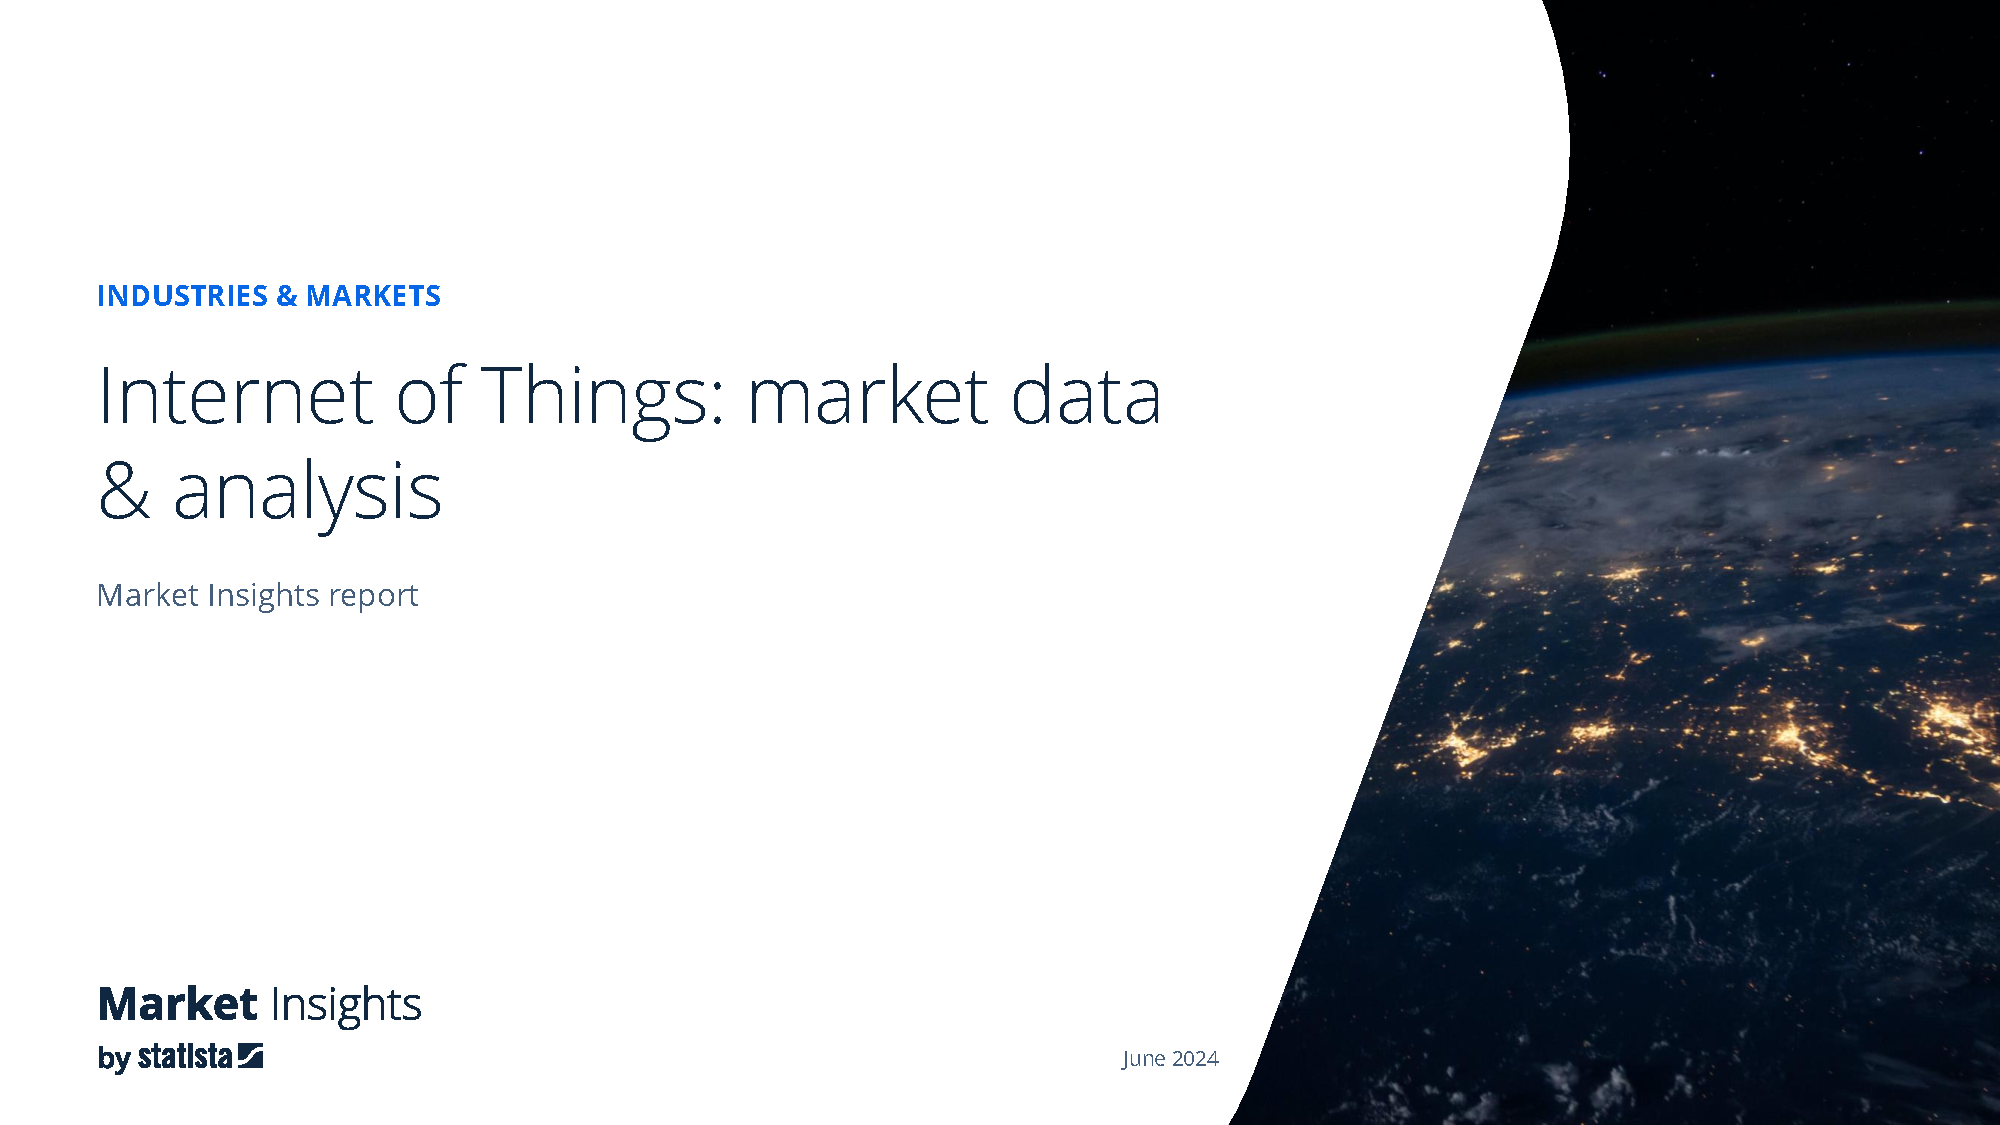
\includegraphics[width=0.85\textwidth]{Statista_iot.png}
\caption{IoT-Verbindungen weltweit}
\end{figure}

Das BSI schreibt in seinem Bericht zur Lage der Internetsicherheit in Deutschland aus dem Jahr 2024: ,,Neben klassischen Bürocomputersystemen können Angreifer auch alle anderen internetfähigen Geräte mit einem Schadprogramm infizieren und in ein Botnetz integrieren. Das betrifft zum Beispiel Geräte wie Smartphones, Tablets, Router oder auch IoT-Geräte wie zum Beispiel Fernseher, Set-Top- Boxen, Webcams etc.''[\cite[15]{BundesamtfurSicherheitinderInformationstechnik.20241125}]
	
	\section{Methodik}
Für die zwei Bereiche der Forschungsfrage werden verschiedene Methodiken angewendet.

Bei der Untersuchung der Liegenschaften wird ein physisches Experiment durchgeführt und anschließend die Daten aus diesem Experiment ausgewertet.

Für die Handlungsempfehlungen und Information findet eine Literaturrecherche statt und falls sich geeignete Interviewpartner finden auch Einzelinterviews.

	
	\section{Gliederung}
Neben den üblichen Bestandteilen einer Abschlussarbeit sind die folgenden Kapitel vorgesehen
\begin{description}
\item[Grundlagen] Die theoretischen Grundlagen werden erarbeitet und technische Prinzipien erklärt
\item[Aufbau des Experiments] Vorstellung des technischen Equipments  
\item[Durchführung des Experiments] Beschreibung der eigentlichen Durchführung des Experiments
\item[Datenauswertung] Auswertung der Daten und Rückschlüsse aus dem Experiment
\item[Experteninterview] Beschreibung und Auswertung der Kernaussagen aus dem oder den Interviews
\item[Handlungsempfehlung für die Hausleitung] Darstellung des Experiments und Handlungsempfehlungen
\item[Handreichung für Mitarbeiter] Ausarbeitung über den Umgang mit IoT-Geräten in der Behörde
\end{description}
	
	\section{Zeitplan}
\begin{description}
\item[12 Wochen vor Abgabe] Anmeldung der Arbeit, erste Literaturrecherche, Anfragen an Interviewpartner
\item[11-10] Literaturrecherche, Erarbeitung von Grundlagen und Interviewfragen
\item[9-6] Vorbereitung, Durchführung und Auswertung des Experiments
\item[5] Späteste Durchführung von Interviews
\item[4-3] Auswertung der Interviews, Schreiben von Informationsmaterial und Handlungsempfehlungen
\item[2] Korrekturlesen
\item[1] Puffer
\item[0] Druck und Abgabe
\end{description}

	\section{Schlussbemerkung}
Das Thema Gefahren des Internet of Things hat durch die stark ansteigende Anzahl an Geräten und Verbindungen ein Risiko- und Sicherheitspotential. Das BSI zeigt dies in seinem jährlich erscheinenden Berichten, zuletzt im Jahr 2024. Durch den einfachen Zugang zu solchen Geräten in Form von Küchenutensilien, Leuchtmitteln und anderen Formen können diese ohne böswillige Absicht in die Arbeitsumgebung der Behörde eingebracht werden. In den Netzwerken der Behörde sind auf Grund seiner Operationen zahlreiche Programmierer und Administratoren aktiv. Entsprechend häufig sind Adminaccounts und es besteht die Gefahr, dass die Geräte in ein Netzwerk eingepflegt wurden oder das sie als Einfallstore zu absichtlichen IoT-Netzwerken in der Behörde benutzt werden.
Dies soll hier erforscht werden und entsprechende Empfehlungen und Informationen erarbeitet werden.

	\nocite{*}
	\printbibliography
\end{document}
